\documentclass[11pt, letterpaper]{article}
\usepackage[utf8]{inputenc}
\usepackage[letterpaper, margin=0.5in]{geometry}
\usepackage{amsmath}
\usepackage{amssymb}
\usepackage{amsthm}
\usepackage{graphicx}
\usepackage{listings}
\usepackage[font=scriptsize]{caption}
\usepackage{subcaption}
\usepackage{xcolor}

\newtheorem{lemma}{Lemma}
\newcommand{\indep}{\perp \!\!\! \perp}

\definecolor{codegreen}{rgb}{0,0.6,0}
\definecolor{codegray}{rgb}{0.5,0.5,0.5}
\definecolor{codepurple}{rgb}{0.58,0,0.82}
\definecolor{backcolour}{rgb}{0.95,0.95,0.92}

\lstdefinestyle{mystyle}{
    backgroundcolor=\color{backcolour},   
    commentstyle=\color{codegreen},
    keywordstyle=\color{magenta},
    numberstyle=\tiny\color{codegray},
    stringstyle=\color{codepurple},
    basicstyle=\ttfamily\footnotesize,
    breakatwhitespace=false,
    texcl=true,
    mathescape=true,
    breaklines=true,                 
    captionpos=b,                    
    keepspaces=true,                 
    numbers=left,                    
    numbersep=5pt,                  
    showspaces=false,                
    showstringspaces=false,
    showtabs=false,                  
    tabsize=2
}

\lstset{style=mystyle}
\graphicspath{ {.} }
\captionsetup{justification=raggedright, singlelinecheck=false}

\author{Ryan Tang}
\title{STA 542 HW 1}
\date{February 9th 2023}

\begin{document}
\maketitle

\section{Ex 1}
We are given a MA(1) model $x_t = \theta w_{t-1} + w_t, \theta=2.3$. Assuming Gaussian noise $w_t \thicksim N(0, v)$. We have the following properties. That any trace $x_{1:n}$ follows a multivariate-normal joint with $0$ mean and tri-diagonal covariance matrix.
\begin{align*}
    x_t &\thicksim N(0, v(1+\theta^2)) \\
    x_{1:n} &\thicksim N(0, \Gamma_n) \\
    \Gamma_n &= v \begin{bmatrix}
        1+\theta^2 & \theta & 0 & \dots & 0 \\
        \theta & 1+\theta^2 & \theta & 0 & \vdots \\
        \vdots & \ddots & \ddots & \ddots & \vdots\\
        \vdots & \dots & \theta & 1+\theta^2 & \theta \\
        0 & \dots & 0 & \theta & 1+\theta^2 \\
    \end{bmatrix} \\
\end{align*}
With this, we can simply read off the ACF.
\begin{align*}
    corr(x_{t+h}, x_t) &= \frac{cov(x_{t_h}, x_t)}{v(1+\theta^2)} \\
        &= \begin{cases}
            1 & h=0 \\
            \frac{\theta}{1+\theta^2} & |h|=1 \\
            0 & |h|>0 \\
        \end{cases}
\end{align*}

To derive the PACF function, it is more involved. The definition of PACF is equalvient to $corr(x_{t+h}, x_t|x_{n/\{t+h, t\}})$ Due to normality, any conditional bi-variate $(x_{t+h}, x_t | x_{n/\{t+h, t\}})$ is also Gaussian. Hence, we can use the block matrix lemma to arrive at the conditional bivariate correlation, PACF.
\begin{align*}
    \Gamma &= \begin{bmatrix} V_1 & R \\ R^{\intercal} & V_2 \end{bmatrix} \\
    K &= \Gamma^{-1} = \begin{bmatrix} K_1 & H \\ H^{\intercal} & K_2 \end{bmatrix} \\
    (x_1 | x_2) &\thicksim N(A_1x_2, K_1^{-1}) \\
    x_1 &= [x_{t+h}, x_t]' \quad\quad x_2 = [x_{t+1}, x_{t+2}, \dots x_{t+h-1}]' \\
    A_ &= RV_2^{-1} \\
    K_1^{-1} &= V_1 - RV_2^{-1}R^{\intercal} \\
    corr(x_{t+h}, x_t|x_{n/\{t+h, t\}}) &= \phi_{hh} = - \frac{(-\theta)^h}{\sum_{i=0}^h \theta^{2i}}
\end{align*}

\newpage
\section{Ex 2}
\paragraph{(a)} Here we plotted the ACF and PACF plots in the hope that we could fit an ARMA model on the series. The PACF indicates a 2-order model $AR(2)$ because most of the terms after lag 2 level off or are insignificant. Of course, it is not entirely correct based on the plot.

\begin{figure*}[!h]
  \centering
  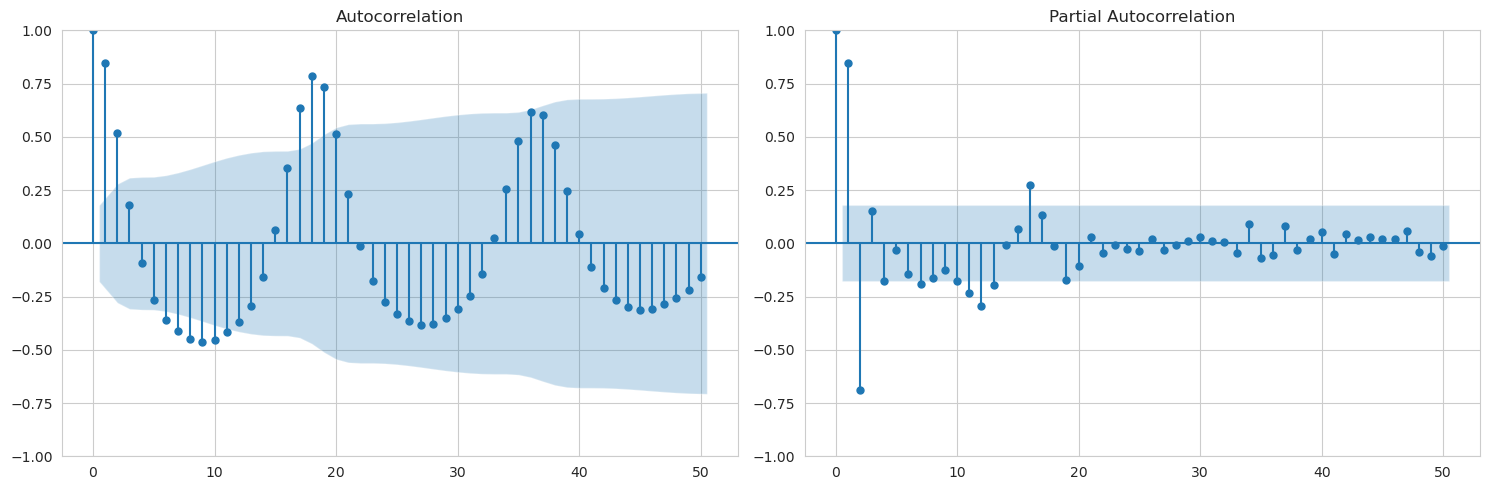
\includegraphics[width=0.9\textwidth]{plot1.png}
  \captionsetup{justification=centering}
  \caption{ACF & PACF plots}
\end{figure*}

\paragraph{(b)} The fitted model provides the following estimated parameters. $\mu=2.8210$, $\phi_1 = 1.5023$, $\phi_2 = -0.7493$, $\sigma^2 = 212.5603$.

\paragraph{(c)} After fitting the $AR(2)$ model using the first 100 data points, we plot the actual series against the simulated one from the fitted model and their corresponding residual plot. We see the simulated trace does poorly, capturing the inherent structure. And the residual certainly doesn't follow the Gaussian white noise assumption.
\begin{figure*}[!h]
  \centering
  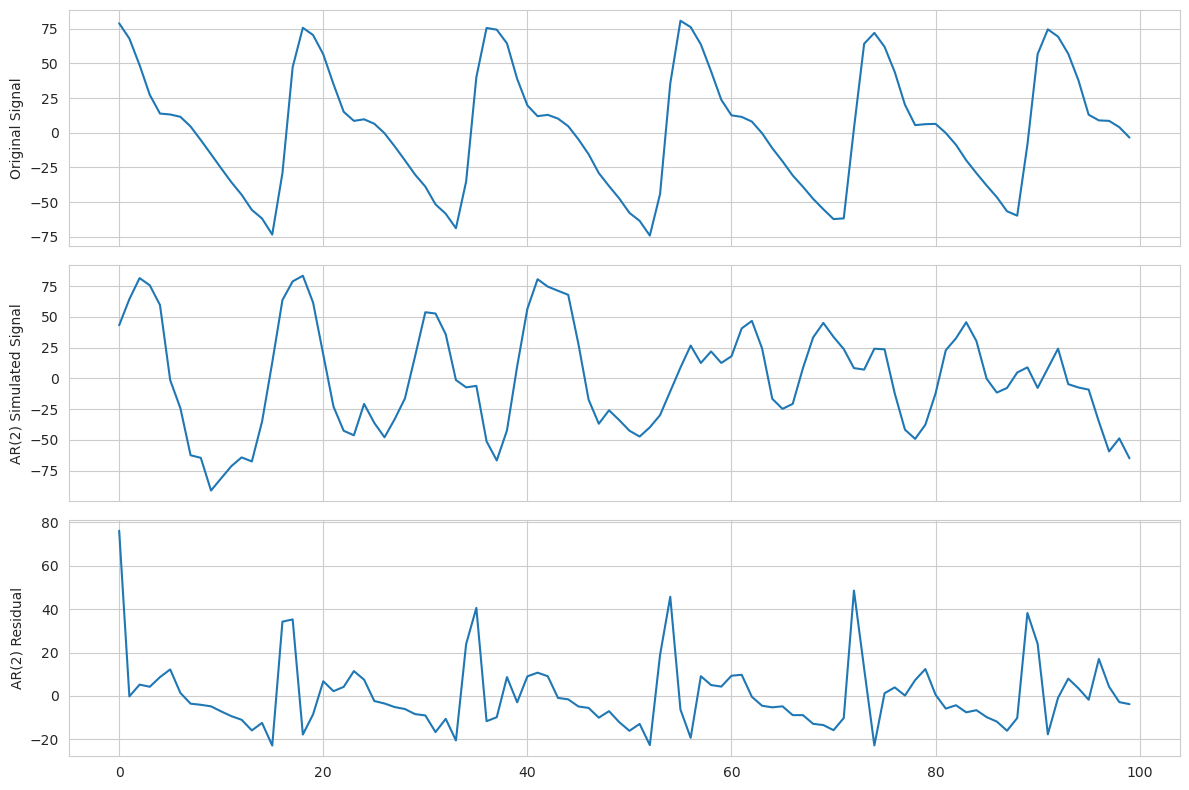
\includegraphics[width=0.8\textwidth]{plot2.png}
  \captionsetup{justification=centering}
  \caption{Simulated vs the truth signal & residual plots}
\end{figure*}

\paragraph{(d - e)} To investigate further, we conducted a forecast for the rest of the remaining 20 unseen data points and plotted them against each other. The 95\% forecast confidence interval is also provided under the shaded grey area. Unfortunately, the forecast is too bad to comment on. It literally just made the $sigma^2$ so large that it covers the entire historical range and the mean estimate as close as 0. I don't believe AR is an ideal model for this dataset. The trace has more structure than noise, to be honest. And $AR(.)$ is not good at such task solely based on the observation.

\begin{figure*}[!h]
  \centering
  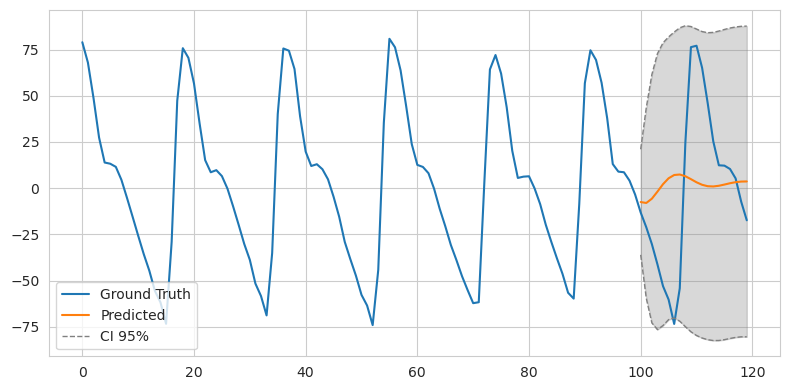
\includegraphics[width=0.8\textwidth]{plot3.png}
  \captionsetup{justification=centering}
  \caption{20 Step ahead forecast with 95\% CI}
\end{figure*}

\end{document}